\documentclass[twoside]{article}
\usepackage{aistats2021}
\usepackage{amsmath, amsfonts, amsthm, amssymb}
\usepackage{graphicx}
\usepackage[colorlinks]{hyperref}
\usepackage[parfill]{parskip}
\usepackage{algpseudocode}
\usepackage{algorithm}
\usepackage{enumerate}
\usepackage[shortlabels]{enumitem}
\usepackage{mathtools}
\usepackage{tikz}
\usepackage{verbatim}

\usepackage{natbib}
\renewcommand{\bibname}{REFERENCES}
\renewcommand{\bibsection}{\subsubsection*{\bibname}}

\DeclareFontFamily{U}{mathx}{\hyphenchar\font45}
\DeclareFontShape{U}{mathx}{m}{n}{<-> mathx10}{}
\DeclareSymbolFont{mathx}{U}{mathx}{m}{n}
\DeclareMathAccent{\wb}{0}{mathx}{"73}

\DeclarePairedDelimiterX{\norm}[1]{\lVert}{\rVert}{#1}
\DeclarePairedDelimiterX{\seminorm}[1]{\lvert}{\rvert}{#1}

% Make a widecheck symbol (thanks, Stack Exchange!)
\DeclareFontFamily{U}{mathx}{\hyphenchar\font45}
\DeclareFontShape{U}{mathx}{m}{n}{
	<5> <6> <7> <8> <9> <10>
	<10.95> <12> <14.4> <17.28> <20.74> <24.88>
	mathx10
}{}
\DeclareSymbolFont{mathx}{U}{mathx}{m}{n}
\DeclareFontSubstitution{U}{mathx}{m}{n}
\DeclareMathAccent{\widecheck}{0}{mathx}{"71}
% widecheck made

\newcommand{\eqdist}{\ensuremath{\stackrel{d}{=}}}
\newcommand{\Graph}{\mathcal{G}}
\newcommand{\Reals}{\mathbb{R}}
\newcommand{\iid}{\overset{\text{i.i.d}}{\sim}}
\newcommand{\convprob}{\overset{p}{\to}}
\newcommand{\convdist}{\overset{w}{\to}}
\newcommand{\Expect}[1]{\mathbb{E}\left[ #1 \right]}
\newcommand{\Risk}[2][P]{\mathcal{R}_{#1}\left[ #2 \right]}
\newcommand{\Prob}[1]{\mathbb{P}\left( #1 \right)}
\newcommand{\iset}{\mathbf{i}}
\newcommand{\jset}{\mathbf{j}}
\newcommand{\myexp}[1]{\exp \{ #1 \}}
\newcommand{\abs}[1]{\left \lvert #1 \right \rvert}
\newcommand{\restr}[2]{\ensuremath{\left.#1\right|_{#2}}}
\newcommand{\ext}[1]{\widetilde{#1}}
\newcommand{\set}[1]{\left\{#1\right\}}
\newcommand{\seq}[1]{\set{#1}_{n \in \N}}
\newcommand{\floor}[1]{\left\lfloor #1 \right\rfloor}
\newcommand{\Var}{\mathrm{Var}}
\newcommand{\Cov}{\mathrm{Cov}}
\newcommand{\diam}{\mathrm{diam}}

\newcommand{\emC}{C_n}
\newcommand{\emCpr}{C'_n}
\newcommand{\emCthick}{C^{\sigma}_n}
\newcommand{\emCprthick}{C'^{\sigma}_n}
\newcommand{\emS}{S^{\sigma}_n}
\newcommand{\estC}{\widehat{C}_n}
\newcommand{\hC}{\hat{C^{\sigma}_n}}
\newcommand{\vol}{\text{vol}}
\newcommand{\spansp}{\mathrm{span}~}
\newcommand{\1}{\mathbf{1}}

\newcommand{\Linv}{L^{\dagger}}
\DeclareMathOperator*{\argmin}{argmin}
\DeclareMathOperator*{\argmax}{argmax}

\newcommand{\emF}{\mathbb{F}_n}
\newcommand{\emG}{\mathbb{G}_n}
\newcommand{\emP}{\mathbb{P}_n}
\newcommand{\F}{\mathcal{F}}
\newcommand{\D}{\mathcal{D}}
\newcommand{\R}{\mathcal{R}}
\newcommand{\Rd}{\Reals^d}
\newcommand{\Nbb}{\mathbb{N}}

%%% Vectors
\newcommand{\thetast}{\theta^{\star}}
\newcommand{\betap}{\beta^{(p)}}
\newcommand{\betaq}{\beta^{(q)}}
\newcommand{\vardeltapq}{\varDelta^{(p,q)}}
\newcommand{\lambdavec}{\boldsymbol{\lambda}}

%%% Matrices
\newcommand{\X}{X} % no bold
\newcommand{\Y}{Y} % no bold
\newcommand{\Z}{Z} % no bold
\newcommand{\Lgrid}{L_{\grid}}
\newcommand{\Dgrid}{D_{\grid}}
\newcommand{\Linvgrid}{L_{\grid}^{\dagger}}
\newcommand{\Lap}{L}
\newcommand{\NLap}{{\bf N}}
\newcommand{\PLap}{{\bf P}}
\newcommand{\Id}{I}

%%% Sets and classes
\newcommand{\Xset}{\mathcal{X}}
\newcommand{\Vset}{\mathcal{V}}
\newcommand{\Sset}{\mathcal{S}}
\newcommand{\Hclass}{\mathcal{H}}
\newcommand{\Pclass}{\mathcal{P}}
\newcommand{\Leb}{L}
\newcommand{\mc}[1]{\mathcal{#1}}

%%% Distributions and related quantities
\newcommand{\Pbb}{\mathbb{P}}
\newcommand{\Ebb}{\mathbb{E}}
\newcommand{\Qbb}{\mathbb{Q}}
\newcommand{\Ibb}{\mathbb{I}}

%%% Operators
\newcommand{\Tadj}{T^{\star}}
\newcommand{\dive}{\mathrm{div}}
\newcommand{\dif}{\mathop{}\!\mathrm{d}}
\newcommand{\gradient}{\mathcal{D}}
\newcommand{\Hessian}{\mathcal{D}^2}
\newcommand{\dotp}[2]{\langle #1, #2 \rangle}
\newcommand{\Dotp}[2]{\Bigl\langle #1, #2 \Bigr\rangle}

%%% Misc
\newcommand{\grid}{\mathrm{grid}}
\newcommand{\critr}{R_n}
\newcommand{\dx}{\,dx}
\newcommand{\dy}{\,dy}
\newcommand{\dr}{\,dr}
\newcommand{\dxpr}{\,dx'}
\newcommand{\dypr}{\,dy'}
\newcommand{\wt}[1]{\widetilde{#1}}
\newcommand{\wh}[1]{\widehat{#1}}
\newcommand{\ol}[1]{\overline{#1}}
\newcommand{\spec}{\mathrm{spec}}
\newcommand{\LE}{\mathrm{LE}}
\newcommand{\LS}{\mathrm{LS}}
\newcommand{\SM}{\mathrm{SM}}
\newcommand{\OS}{\mathrm{OS}}
\newcommand{\PLS}{\mathrm{PLS}}

%%% Order of magnitude
\newcommand{\soom}{\sim}

%%% Theorem environments
\newtheorem{theorem}{Theorem}
\newtheorem{conjecture}{Conjecture}
\newtheorem{lemma}{Lemma}
\newtheorem{example}{Example}
\newtheorem{corollary}{Corollary}
\newtheorem{proposition}{Proposition}
\newtheorem{assumption}{Assumption}
\newtheorem{remark}{Remark}


\theoremstyle{definition}
\newtheorem{definition}{Definition}[section]

\theoremstyle{remark}


\begin{document}
	
\twocolumn[

	\aistatstitle{Minimax Optimal Regression over Sobolev Spaces via Laplacian Regularization on Neighborhood Graphs}
	
	\aistatsauthor{Alden Green, Sivaraman Balakrishnan, and Ryan J. Tibshirani}

	\aistatsaddress{Carnegie Mellon University}]
	

\begin{abstract}
	In this paper we study the statistical properties of Laplacian smoothing, a graph-based approach to non-parametric regression. Under standard regularity conditions, we establish upper bounds on the error of the Laplacian smoothing estimator $\wh{f}$, and a goodness-of-fit test based on $\wh{f}$. These upper bounds match the minimax optimal estimation and testing rates of convergence over the first-order Sobolev class $H^1(\Xset)$, where $\Xset \subset \Rd$ and $1 \leq d < 4$; in the estimation problem, they are within a $\log n$ factor of optimal when $d = 4$. Additionally, we prove that Laplacian smoothing is manifold adaptive: if $\Xset$ is an $m$ dimensional manifold embedded in $\Reals^d$ with $m \ll d$, then the error rate of Laplacian smoothing methods depends only on the intrinsic dimension $m$ and not on the ambient dimension $d$. 
\end{abstract}

\section{INTRODUCTION}
In the nonparametric regression problem, we observe samples $(X_1,Y_1),\ldots,(X_n,Y_n)$ according to the signal plus noise model
\begin{equation}
\label{eqn:signal_plus_noise_model}
Y_i = f_{0}(X_i) + \varepsilon_i,
\end{equation}
with $\varepsilon_i \sim N(0,1)$ independent Gaussian noise. Our goal is to perform statistical inference on the unknown regression function $f_0$, by which we mean either \emph{estimating} $f_0$ or more simply \emph{testing} whether $f_0 = 0$, i.e whether there is any signal present. 

The Laplacian smoothing estimator $\wh{f}$ \citep{smola2003} is a penalized least squares estimator, defined on a graph. Letting $G = \bigl(\{1,\ldots,n\},W\bigr)$ be a weighted graph over vertices $\{1,\ldots,n\}$ which we associate with the sample points $\{X_1,\ldots,X_n\}$, the estimator $\wh{f}$ is given by
\begin{equation}
\label{eqn:laplacian_smoothing}
\wh{f} :=  \min_{f \in \Reals^n} \biggl\{\sum_{i = 1}^{n}(Y_i - f_i)^2 + \rho \cdot f^T \Lap f \biggr\}.
\end{equation}
Here $\Lap$ is the graph Laplacian matrix (defined in Section~\ref{sec:problem_setup_and_background}), $G$ is typically a geometric graph (such as a $k$NN or neighborhood graph) and the penalty
\begin{equation*}
f^T \Lap f = \frac{1}{2} \sum_{i,j = 1}^{n} W_{ij}\bigl(f_i - f_j\bigr)^2
\end{equation*}
thus encourages $\wh{f}_i \approx \wh{f}_j$ when $X_i \approx X_j$. Assuming~\eqref{eqn:laplacian_smoothing} is a reasonable estimator of $f_0$, the statistic
\begin{equation}
\label{eqn:laplacian_smoothing_test}
\wh{T} := \frac{1}{n}\bigl\|\wh{f}\bigr\|_2^2 
\end{equation}
is in turn a reasonable way to decide if $f_0 = 0$. 

Of course there exist many methods for nonparametric regression \citep{gyorfi2006,wasserman2006,tsybakov2008_book}, but Laplacian smoothing has its own set of advantages. For instance:
\begin{itemize}
	\item \emph{Computational ease.} Laplacian smoothing is fast, easy, and stable to compute. The estimate $\wh{f}$ can be computed by solving a symmetric, diagonally dominant linear system. There are known extremely fast and reliable solvers for exactly this problem (see e.g. the seminal papers of \cite{spielman2011,spielman2013,spielman2014}, or the monograph by~\cite{vishnoi2012} and references therein).
	\item \emph{Generality.} Laplacian smoothing is well defined whenever one can associate a graph with some observed responses. This generality lends itself to many different data modalities: for instance text and image classification, to name only two \citep{kondor2002, belkin03a,belkin2006}. 
	\item \emph{Weak supervision.} Although we study Laplacian smoothing in the supervised learning setup~\eqref{eqn:signal_plus_noise_model}, it can be easily adapted to the semi-supervised or unsupervised settings \citep{nadler09,slepcev17,dunlop2020,calder2019b}.
\end{itemize}

For these reasons, a body of work has emerged analyzing the statistical properties of Laplacian smoothing, and graph-based methods more generally. Roughly speaking, these works can be divided into two categories, based on the perspective they adopt. 
\begin{itemize}
	\item In the \emph{fixed design perspective}, the design points $\{X_1,\ldots,X_n\}$ and the graph $G$ are treated as fixed, and inference is carried out on the evaluations $\bigl(f_0(X_1),\ldots,f_0(X_n)\bigr) \in \Reals^n$.\footnote{To be clear, while in this setting $G$ may be a geometric graph, in principle it could be any graph over $\{1,\ldots,n\}$.} In this context, tight upper bounds have been derived on the error of graph-based estimators \citep{wang2016, sadhanala16,sadhanala17,kirichenko2017,kirichenko2018} and tests \citep{sharpnack2013,sharpnack2013b,sharpnack2015}, which certify that such procedures are \emph{optimal} over ``function'' classes $\mc{F} \subseteq \Reals^n$. The downside of this work is that it may be unnatural to assume a priori that the graph $G$ is fixed, or that the evaluations $\bigl(f_0(X_1),\ldots,f_0(X_n)\bigr)$ belong to some discrete ``function'' class.
	\item In the arguably more natural \emph{random design perspective},  one assumes the design points $X_1,\ldots,X_n$ are sampled independently from some distribution $P$ supported on a domain $\Xset \subset \Rd$. Inference is drawn on the regression function $f_0: \Xset \to \Reals$, which is typically assumed to be smooth in some continuum sense, e.g. it possesses a first derivative bounded in $L^{\infty}$ (H\"{o}lder) or $\Leb^2$ (Sobolev) norm. To conduct graph-based inference, the user first builds a neighborhood graph over the random design points---so that $W_{ij}$ is large iff $X_i$ and $X_j$ are close in say Euclidean distance---and then solves e.g.~\eqref{eqn:laplacian_smoothing} or~\eqref{eqn:laplacian_smoothing_test}. In this context, various graph-based procedures have been shown to be \emph{consistent}: as $n \to \infty$, they converge to a \emph{continuum} limit (see \citep{belkin07,trillos2018,vonluxburg2008} among others). However, until recently such statements were not accompanied by error rates, and such error rates as have been proved \citep{lee2016,trillos2020} are not optimal over continuum function spaces, such as H\"{o}lder or Sobolev classes. 
\end{itemize}
Hereafter, we will adopt the random design perspective, and seek to answer the following question:
\begin{quote}{When $f_0$ is assumed to smooth in a continuum sense, does Laplacian smoothing achieve optimal performance for estimation and goodness-of-fit testing?} 
\end{quote}
On the one hand, this is no small question---rather, it is arguably the fundamental question of nonparametric regression, and without an answer one cannot fully compare the statistical properties of Laplacian smoothing to its competitors. On the other hand, it seems difficult to answer: there is a fundamental gap between the \emph{discrete} smoothness imposed by the penalty $f^T \Lap f$ in~\eqref{eqn:laplacian_smoothing} and the \emph{continuum} smoothness assumed on $f_0$, and to obtain sharp upper bounds we will need to bridge this gap in a tight sense.

\section{SUMMARY OF RESULTS}

\paragraph{Advantages of the discrete approach.} In light of this last point, it is worth asking whether there is any \emph{statistical} advantage to solving a discrete problem such as~\eqref{eqn:laplacian_smoothing} (setting aside computational considerations for the moment). After all, we could have instead solved the following variational problem:
\begin{equation}
\label{eqn:thin_plate_spline}
\wt{f} := \argmin_{f} \biggl\{\sum_{i = 1}^{n} \bigl(Y_i - f(X_i)\bigr)^2 + \rho \cdot \int_{\Xset} \|\nabla f(x)\|^2 \,dx \biggr\},
\end{equation}
with the minimum computed over all functions $f$ for which the criterion is finite--or used the statistic
\begin{equation}
\label{eqn:thin_plate_spline_test}
\wt{T} := \|\wt{f}\|_n^2.
\end{equation}
The penalty in~\eqref{eqn:thin_plate_spline} leverages the assumption that $f_0$ possesses a bounded derivative in a seemingly natural manner. Indeed, for this reason the estimator $\wt{f}$ (and to a lesser extent, the statistic $\wt{T}$) are well known--- in the univariate case, $\wt{f}$ is simply a \emph{smoothing spline}, and when $d > 1$ it is an example of a \emph{thin-plate spline}---and their statistical properties are well-understood \citep{vandergeer2000, liu2019}. Moreover, there exist strong connections between smoothing/thin-plate splines and Laplacian smoothing: as we show later on in~\eqref{eqn:seminorm_consistency}, in a certain sense the Laplacian smoothing problem~\eqref{eqn:laplacian_smoothing} can be seen as a discrete and noisy approximation to~\eqref{eqn:thin_plate_spline}. At first blush, this suggests that Laplacian smoothing should at best inherit the statistical properties of smoothing/thin-plate splines, and at worst may have meaningfully larger error.

However, as we shall see the actual story is quite different: remarkably, Laplacian smoothing enjoys optimality properties in cases where the thin-plate spline problem~\eqref{eqn:thin_plate_spline} is not even well-posed. Tables~\ref{tbl:estimation_rates} and~\ref{tbl:testing_rates} summarize the gap. As we establish in Theorems~\ref{thm:laplacian_smoothing_estimation1}-\ref{thm:laplacian_smoothing_testing_manifold}, when computed over an appropriately formed neighborhood graph, Laplacian smoothing estimators and tests are minimax optimal over first-order \emph{continuum} Sobolev balls. This holds true either when $\Xset \subset \Rd$ is a full-dimensional domain and $d = 1,2$ or $3$, or when $\Xset$ is a submanifold of $\Rd$ of intrinsic dimension $m = 1,2,$ or $3$. Additionally, the estimator $\wh{f}$ is nearly minimax optimal (to within a $(\log n)^{1/3}$ factor) when $d$ (or $m$) = $4$. By contrast, smoothing splines are optimal only when $d$ (or $m$) = $1$. In higher dimensions, technically speaking the problem~\eqref{eqn:thin_plate_spline} is not even well-posed, and any practical implementation of the estimator $\wt{f}$ will be inconsistent \citep{green93}. Hence, our results favorably distinguish Laplacian smoothing methods from their natural variational alternatives.
\begin{table}
	\begin{center}
		\begin{tabular}{p{.1\textwidth} | p{.14\textwidth} p{.12\textwidth} }
			Dimension & Laplacian smoothing \eqref{eqn:laplacian_smoothing} & Thin-plate splines \eqref{eqn:thin_plate_spline} \\
			\hline
			$d = 1$ & ${\bf n^{-2/3}}$ & \textcolor{red}{${\bf n^{-2/3}}$} \\
			$d = 2,3$ & ${\bf n^{-2/(2 + d)}}$ & \textcolor{red}{$1$} \\
			$d = 4$ & ${\bf n^{-1/3}} (\log n)^{1/3}$ & \textcolor{red}{$1$} \\
			$d \geq 5$  & $(\log n/n)^{4/(3d)}$ &\textcolor{red}{$1$} \\
		\end{tabular}
	\end{center}
	\caption{Summary of estimation rates over first-order Sobolev balls. Rates in black are new results of this paper, and bolded rates are minimax optimal. Although we suppress it for conciseness, in all cases the dependence of the error rate on the radius of the Sobolev ball is also optimal. For thin-plate splines, ``\textcolor{red}{$1$}'' indicates that the estimator is inconsistent. When $\Xset$ is an $m$ dimensional manifold embedded in $\Rd$, all rates hold with $d$ replaced by $m$, without any change in the method in the case of Laplacian smoothing.}
	\label{tbl:estimation_rates}
\end{table}

\begin{table}
	\begin{center}
		\begin{tabular}{p{.1\textwidth} | p{.14\textwidth} p{.12\textwidth} }
			Dimension & Laplacian smoothing \eqref{eqn:laplacian_smoothing_test} & Thin-plate splines \eqref{eqn:thin_plate_spline_test} \\
			\hline
			$d = 1$ & ${\bf n^{-4/5}}$ & \textcolor{red}{${\bf n^{-4/5}}$} \\
			$d = 2,3$ & ${\bf n^{-4/(4 + d)}}$ & \textcolor{red}{$n^{-1/2}$} \\
			$d \geq 4$\footnotemark & ${ \bf n^{-1/2}}$ & \textcolor{red}{${ \bf n^{-1/2}}$}
		\end{tabular}
	\end{center}
	\caption{Summary of testing rates over fixed radius first-order Sobolev balls; black, red, and bold font used as in Table~\ref{tbl:estimation_rates}. Rates for $d \geq 4$ assume $f_0 \in \Leb^4(\Xset,M)$. When $\Xset$ is an $m$ dimensional manifold embedded in $\Rd$, all rates hold with $d$ replaced by $m$.}
	\label{tbl:testing_rates}
\end{table}
\footnotetext{Assuming $f_0 \in \Leb^4(\Xset,M)$.}
\paragraph{Future extensions.}
To be clear, these results are not the end of the story. For one thing, the estimator $\wh{f}$ is defined only at the design points $\{X_1,\ldots,X_n\}$. As such, we measure loss using the in-sample mean squared error 
\begin{equation*}
\|\wh{f} - f_0\|_n^2 := \frac{1}{n}\sum_{i = 1}^{n} \Bigl(\wh{f}_i - f_0(X_i)\Bigr)^2.
\end{equation*}
In Section~\ref{sec:minimax_optimal_laplacian_smoothing}, we briefly discuss how one could extend $\wh{f}$ to a function over all $\Xset$, in such a way that the out-of-sample mean square error $\|\wh{f} - f_0\|_{\Leb^2(\Xset)}$ remains small, but leave a formal analysis of the problem to future work.

In a different direction, the problem~\eqref{eqn:thin_plate_spline} is only a special, first-order case of thin-plate splines. In general, the degree-$k$ thin plate spline is defined as a minimizer of
\begin{equation*}
\sum_{i = 1}^{n} (Y_i - f(X_i))^2 + \rho \cdot \sum_{|m| = k} \int_{\Xset} \bigl(D^mf(x)\bigr)^2 \,dx
\end{equation*}
where for each multiindex $m$ we write $D^m$ for the partial derivative $D^mf(x):= \partial^kf/\partial x_{1}^{m_1}\ldots \partial x_{d}^{m_d}$. Assuming the $k$th-order partial derivatives $D^mf_0$ are all bounded in $\Leb^2(\Xset)$ norm, the degree-$k$ thin plate spline has error on the order of $n^{-2k/(2k + d)}$ \citep{vandergeer2000}, which is the minimax optimal rate for such functions. Of course, assuming $f_0$ possesses $k$ bounded derivatives for some $2k > d$ is a rather strong assumption which may not be warranted, but at present we do not know whether (adaptations of) Laplacian smoothing on neighborhood graphs can achieve these faster rates.

% \paragraph{Notation.}
% AJG: Need to make sure these are all defined somewhere
% For an integer $p > 0$, we use $\Leb^p(\Xset)$ to refer to the set of functions $f$ for which the $p$th moment $\norm{f}_{\Leb^p(\Xset)}^p := \int_{\Xset} |f(x)|^p \,dx < \infty$, and $C^p(\Xset)$ to refer to those function which are $p$-times continuously differentiable with bounded $p$th derivative. Finally, we use $C,C_1,\ldots$ and $c,c_1,\ldots$ as constants which are independent of $n$ and $f_0$, and for convenience, we will also use asymptotic notation: $a_n \lesssim b_n$ means that $a_n \leq Cb_n$ for some $C > 0$, and $a_n \asymp b_n$ means that $a_n \lesssim b_n$ and $b_n \lesssim a_n$.

\section{BACKGROUND}
\label{sec:problem_setup_and_background}
Before we formally state our main results in Section~\ref{sec:minimax_optimal_laplacian_smoothing}, we define neighborhood graph Laplacians, and review the known minimax rates over first-order Sobolev spaces.

\paragraph{Neighborhood graph Laplacians.}
As mentioned, in the graph-based approach to nonparametric regression we first build a neighborhood graph $G_{n,r} = ([n],W)$ which captures the geometry of $P$ and $\mc{X}$ in an appropriate sense. The $n \times n$ weight matrix $W = (W_{ij})$ encodes proximity between pairs of samples; for a kernel function $K: [0,\infty) \to \Reals$ and connectivity radius $r > 0$, the entries $W_{ij}$ are given by
\begin{equation*}
\label{eqn:neighborhood_graph}
W_{ij} = K\Biggl(\frac{\norm{X_i - X_j}}{r}\Biggr),
\end{equation*}
where $\norm{\cdot}$ is the Euclidean norm in $\Rd$. Then the degree matrix $D$ is the $n \times n$ diagonal matrix with entries $D_{ii} = \sum_{j = 1}^{n}W_{ij}$, and the graph Laplacian can be written as
\begin{equation}
\label{eqn:graph_Laplacian}
\Lap_{n,r} = D - W;
\end{equation}
we add the subscripts $n$ and $r$ to $\Lap$ and $G$ to emphasize that they depend on the random design points $X_1,\ldots,X_n$ and the radius $r$. To avoid any confusion: henceforth when speak of $\wh{f}$ and $\wh{T}$, we will always assume they are fit using the neighborhood graph Laplacian $L = L_{n,r}$. 

Note that $L$ is a symmetric, positive semi-definite matrix, and so admits an eigendecomposition $L = \sum_{k = 1}^{n} \lambda_k v_k v_k^T$. We order the eigenvalues $0 = \lambda_1 \leq \lambda_2 \leq \cdots \leq \lambda_n$, and always consider unit-norm eigenvectors $\|v_k\|_2^2 = 1$; we will make reference to these objects later on.

\paragraph{Sobolev spaces.}
Now that we've defined the neighborhood graph Laplacian $\Lap_{n,r}$, we step away from graph-based methods for a moment, to briefly recall some classical results regarding minimax rates over Sobolev classes.

We say that a function $f \in \Leb^2(\Xset)$ belongs to the \emph{first-order Sobolev space} $H^1(\Xset)$ iff for each $j = 1,\ldots,d$, the weak partial derivative $D^jf$ exists and belong to $\Leb^2(\Xset)$. For such functions $f \in H^1(\Xset)$, the Sobolev seminorm $\seminorm{f}_{H^{1}(\Xset)}$ is the average size of the gradient;
\begin{equation*}
\seminorm{f}_{H^1(\Xset)}^2 = \int_{\Xset} \bigl\|\nabla f(x)\bigr\|^2 \,dx
\end{equation*}
with corresponding Sobolev norm $\norm{f}_{H^1(\Xset)} := \norm{f}_{\Leb^2(\Xset)} + |f|_{H^1(\Xset)}$. The Sobolev balls $H^1(\Xset,M)$ for $M > 0$ are then defined as
\begin{equation*}
H^1(\Xset,M) := \Bigl\{f \in H^1(\Xset): \norm{f}_{H^1(\Xset)}^2 \leq M^2\Bigr\}.
\end{equation*}
For further details regarding Sobolev spaces see e.g.~\citep{evans10,leoni2017}.

\paragraph{Minimax rates.}
To carry out a minimax analysis of regression in Sobolev spaces, one must impose some regularity conditions on the design distribution $P$. We shall assume the following.
\begin{enumerate}[label=(P\arabic*)]
	\item
	\label{asmp:domain}
	$P$ is supported on a domain $\Xset \subset \Rd$, an open, connected set with Lipschitz boundary.
	\item
	\label{asmp:bounded_lipschitz_density} 
	$P$ admits a density $p$ bounded away from $0$ and $\infty$, i.e.
	\begin{equation*}
	0 < p_{\min} \leq p(x) \leq p_{\max} < \infty,~~\textrm{for all $x \in \Xset$.}
	\end{equation*}
	Additionally, the restriction of $p$ to $\Xset$ is Lipschitz, with Lipschitz constant $L_p$.
\end{enumerate}

Under~\ref{asmp:domain} and~\ref{asmp:bounded_lipschitz_density}, the minimax estimation rate over Sobolev balls is (see e.g. \citep{tsybakov2008_book}),
\begin{equation}
\label{eqn:sobolev_space_estimation_minimax_rate}
\inf_{\wh{f}} \sup_{f_0 \in H^1(\Xset, M)} \Ebb\Bigl[\norm{\wh{f} - f_0}_{L^2(\Xset)}^2\Bigr] \asymp M^{2d/(2 + d)}n^{-2/(2 + d)}.
\end{equation}

As nonparametric hypothesis testing is (comparatively) less familiar than nonparametric estimation, we briefly summarize the main idea before stating the optimal error rate. In the goodness-of-fit testing problem, we ask for a test function---formally, a Borel measurable function $\phi$ that takes values in $\{0,1\}$--- which can distinguish between the hypotheses
\begin{equation}
\mathbf{H}_0: f_0 = f_0^{\star}, ~~\textrm{versus}~~ \mathbf{H}_a: f_0 \in \mc{F} \setminus \{f_0^{\star}\}.
\end{equation} 
Typically, the null hypothesis $f_0 = f_0^{\star} \in \mc{F}$ reflects the absence of interesting structure, and $\mc{F} \setminus  \{f_0^{\star}\}$ is a set of smooth departures from this null. To fix ideas, as in \cite{ingster2009} we focus on the problem of \emph{signal detection} in Sobolev spaces, where $f_0^{\star} = 0$ and $\mc{F} = H^1(\Xset,M)$ is a first-order Sobolev ball; this is without loss of generality.

The minimax critical radius is the smallest value of $\epsilon$ such that some level-${\alpha}$ test $\phi$ has power at least $1 - \alpha$ over all $\mc{F}_{\epsilon} := \mc{F} \cap \{f: \|f\|_{\Leb^2(\Xset)} \geq \epsilon\}$:
\begin{equation*}
\epsilon(\mc{F}) := \inf\Biggl\{\epsilon > 0: \inf_{\phi} \biggl[ \sup_{f_0 \in \mc{F}_{\epsilon}} \Ebb_{f_0}[1 - \phi]\biggr] \leq \alpha\Biggr\}
\end{equation*} 
where in the above the infimum is over all level-$\alpha$ tests $\phi$, and $\Ebb_{f_0}[\cdot]$ is the expectation under the regression function $f_0$.\footnote{ Clearly, the minimax critical radius $\epsilon$ depends on $\alpha$. However we adopt the typical convention of treating $\alpha$ as a small but fixed positive constant; hence it will not affect the testing error rates, and we suppress it notationally.} See \citep{ingster82, ingster87, ingster2012} for a more extended treatment of the minimax paradigm in nonparametric testing. 

Testing whether a regression function $f_0$ is equal to $0$ is an easier problem than estimating $f_0$, and so the minimax testing critical radius over $H^1(\Xset,M)$ is much smaller than the minimax estimation rate \citep{ingster2009}:
\begin{equation}
\label{eqn:sobolev_space_testing_critical_radius}
\epsilon^2\Bigl(H^1(\Xset,M)\Bigr) \asymp M^{2d/(4 + d)}n^{-4/(4 + d)}~~\textrm{for $1 \leq d < 4$.}
\end{equation}
When $d \geq 4$ the functions in $H^1(\Xset)$ are very irregular---formally speaking $H^1(\Xset)$ does not continuously embed into $\Leb^4(\Xset)$ when $d \geq 4$---and the minimax testing rates in this regime are unknown. 

\section{MINIMAX OPTIMALITY OF LAPLACIAN SMOOTHING}
\label{sec:minimax_optimal_laplacian_smoothing}

We now formalize the main conclusions of this work: that Laplacian smoothing methods on neighborhood graphs are minimax rate-optimal over first-order continuum Sobolev classes. Throughout this section, we use $C,C_1,\ldots$ and $c,c_1,\ldots$ to refer to constants which do not depend on $n$ or $f_0$. We will assume~\ref{asmp:domain} and ~\ref{asmp:bounded_lipschitz_density}, and additionally that the kernel $K$ satisfies condition~\ref{asmp:kernel}. 
\begin{enumerate}[label=(K\arabic*)]
	\item
	\label{asmp:kernel}
	$K:[0,\infty) \to [0,\infty)$ is a non-increasing function supported on $[0,1]$, its restriction to $[0,1]$ is Lipschitz, and $K(1) > 0$. Additionally, it is normalized so that
	\begin{equation*}
	\int_{\Reals^d} K\bigl(\norm{z}\bigr) \,dz = 1.
	\end{equation*}
	Let $\sigma_K := \frac{1}{d} \int_{\Rd} \|x\|^2 K(\|x\|) \,dx$.
\end{enumerate}
This is a relatively mild condition: the choice of kernel is under the user's control, and moreover~\ref{asmp:kernel} covers many (though not all) common kernel choices.

\paragraph{Estimation error of Laplacian smoothing.} 
Under these conditions, the Laplacian smoothing estimator $\wh{f}$ achieves, up to constants, the minimax risk $n^{-2/(2 + d)}$ over $H^1(\Xset,M)$. This statement will hold whenever the graph $G_{n,r}$ is computed with radius $r$ in the following range.
\begin{enumerate}[label=(R\arabic*)]
	\setcounter{enumi}{0}
	\item 
	\label{asmp:ls_kernel_radius_estimation}
	The neighborhood graph radius $r$ satisfies
	\begin{equation*}
	C_0\biggl(\frac{\log n}{n}\biggr)^{1/d} \leq r \leq n^{-3/(4 + 2d)} M^{(d - 4)/(4 + 2d)} \wedge c_0.
	\end{equation*}
\end{enumerate}
We comment on~\ref{asmp:ls_kernel_radius_estimation} after stating Theorem~\ref{thm:laplacian_smoothing_estimation1}. The proof of this theorem, as with the proofs of all results in this paper, can be found in the supplementary document.
\begin{theorem}
	\label{thm:laplacian_smoothing_estimation1}
	Let $f_0 \in H^1(\Xset,M)$ with $d < 4$. Suppose that that the neighborhood graph $G_{n,r}$ is computed with a radius $r$ which satisfies~\ref{asmp:ls_kernel_radius_estimation},  and the Laplacian smoothing estimator $\wh{f}$ with $\rho = M^{-4/(2 + d)} (nr^{d + 2})^{-1} n^{-2/(2 + d)}$. With probability at least $1 - \delta -  C_1n\exp(-c_1nr^d) - \exp(-c M^{d/(2d + 4)} n^{d/(2+d)})$, it holds that
	\begin{equation}
	\label{eqn:laplacian_smoothing_estimation1}
	\Bigl\|\wh{f} - f_0\Bigr\|_n^2 \leq \frac{C}{\delta} M^{2d/(2 + d)} n^{-2/(2 + d)}.
	\end{equation}
\end{theorem}
To summarize: when $d = 1,2$ or $3$, with high probability the Laplacian smoothing estimator $\wh{f}$ has in-sample mean squared error within a constant factor of the minimax risk. Some remarks:
\begin{itemize}
	\item The lower bound on $r$ imposed by~\ref{asmp:ls_kernel_radius_estimation} is  compatible with practice, where by far the most common choice of radius is the connectivity threshold $r \asymp (\log(n)/n)^{1/d}$, chosen to make the graph $G_{n,r}$ as sparse as possible while still being connected, for maximum computational efficiency. The upper bound is a bit more mysterious. We need it for technical reasons to ensure that $\wh{f}$ does not overfit, but note that as a practical matter one rarely chooses $r$ to be so large.
	\item It is possible to extend $\wh{f}$ to be defined on all of $\Xset$, and evaluate the error of such an extension in $\Leb^2(\Xset)$ norm. Assuming that the extension of $\wh{f}$ and the regression function $f_0$ are both suitably smooth, tools from empirical process theory (Chapter 14 of \cite{wainwright2019}) or approximation theory (Section 15.5 of \citep{johnstone2011}) should guarantee that the $\Leb^2(\Xset)$ error is not too much greater than its in-sample counterpart. In fact, as we show in our supplementary material, if $f_0$ is Lipschitz smooth and we extend $\wh{f}$ to be piecewise constant over the Voronoi tesselation induced by $X_1,\ldots,X_n$, the out-of-sample error $\|f_0 - \wh{f}\|_{\Leb^2(X)}$ is within a negligible factor of the in-sample error $\|f_0 - \wh{f}\|_n$, but we leave analysis of the Sobolev case to future work.
	\item Under the stronger assumption that $f_0$ is Lipschitz smooth, we can replace the factor of $\delta$ in the high probability bound by the sharper $\delta^2/n$.
\end{itemize} 

When $d = 4$, by setting $r \asymp (\log n/n)^{1/4}$ our analysis results in an upper bound on the mean squared error within a $(\log n)^{1/3}$ factor of the minimax risk, but when $d \geq 5$ our analysis yields upper bounds that are much worse than the minimax rate. This mirrors the conclusions of~\cite{sadhanala16}, who investigate estimation rates of Laplacian smoothing over the $d$-dimensional grid graph. \cite{sadhanala16} argue that their analysis is tight, and that it is the estimator, rather than the analysis, which is deficient when $d \geq 5$. Formally proving such a claim turns out to be harder in the random design setting than in the fixed design setting, and we leave it for future work. 

However, we do investigate the matter empirically. In Figure~\ref{fig:fig1}, we consider the mean squared error of the Laplacian smoothing estimator, for several different values of dimension $d$. Here, $X_1,\ldots,X_n$ are sampled uniformly over $\Xset = [-1,1]^d$, and the regression function $f_0(x) \propto \Pi_{i = 1}^{d} \cos(m \pi x_i)$, where $m = 2$ for $d = 2$, and $m = 1$ for $d \geq 3$. This is a rather smooth regression function, and when $d = 2$ and $d = 3$ empirically Laplacian smoothing appears to achieve or exceed the minimax rate. When $d = 4$ Laplacian smoothing appears modestly suboptimal; this fits with our theoretical upper bound, which includes a $(\log n)^{1/3}$ factor that plays a non-negligible role for these problem sizes. On the other hand, when $d = 5$ Laplacian smoothing seems to be decidedly suboptimal. 

\begin{figure}[thb]
	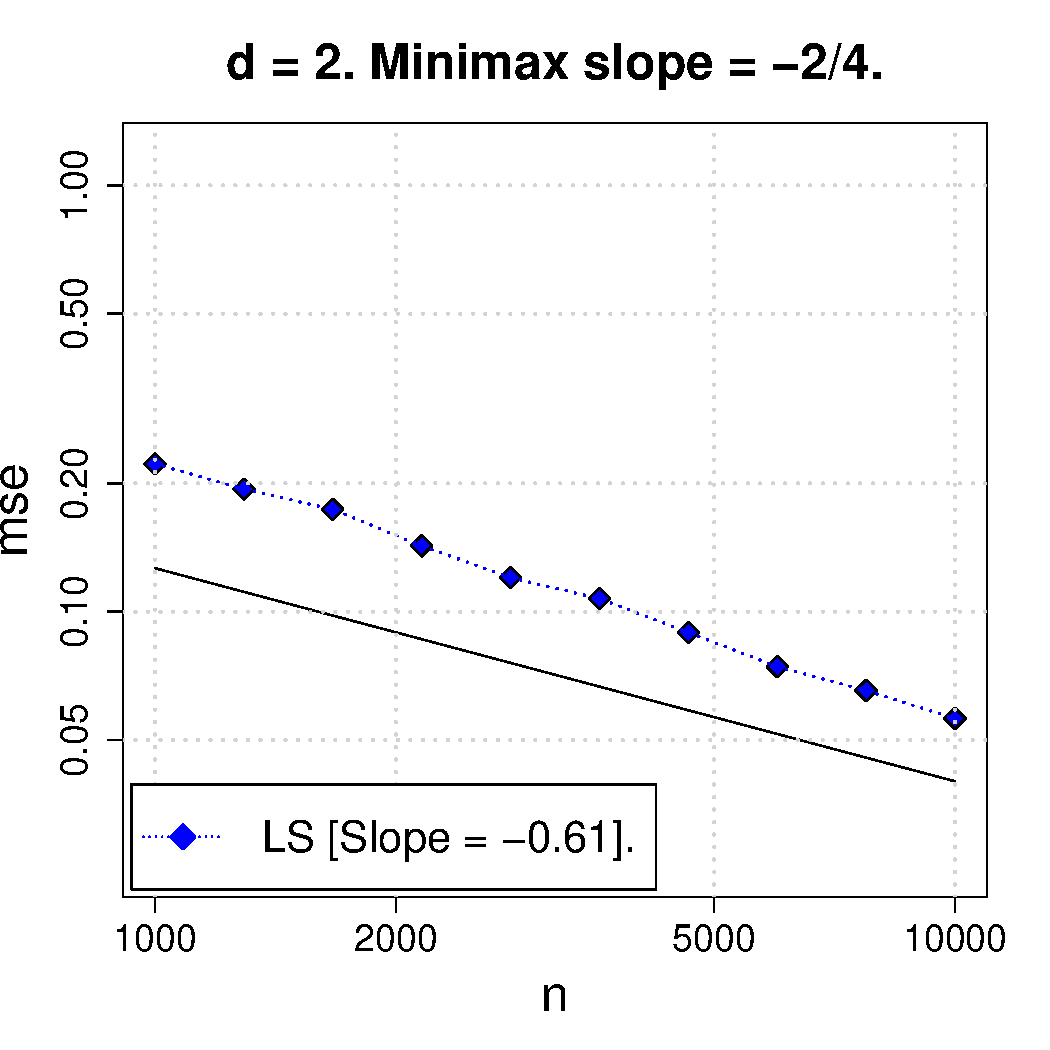
\includegraphics[width=.23\textwidth]{figures/cosine/mse_by_sample_size_2d.pdf}
	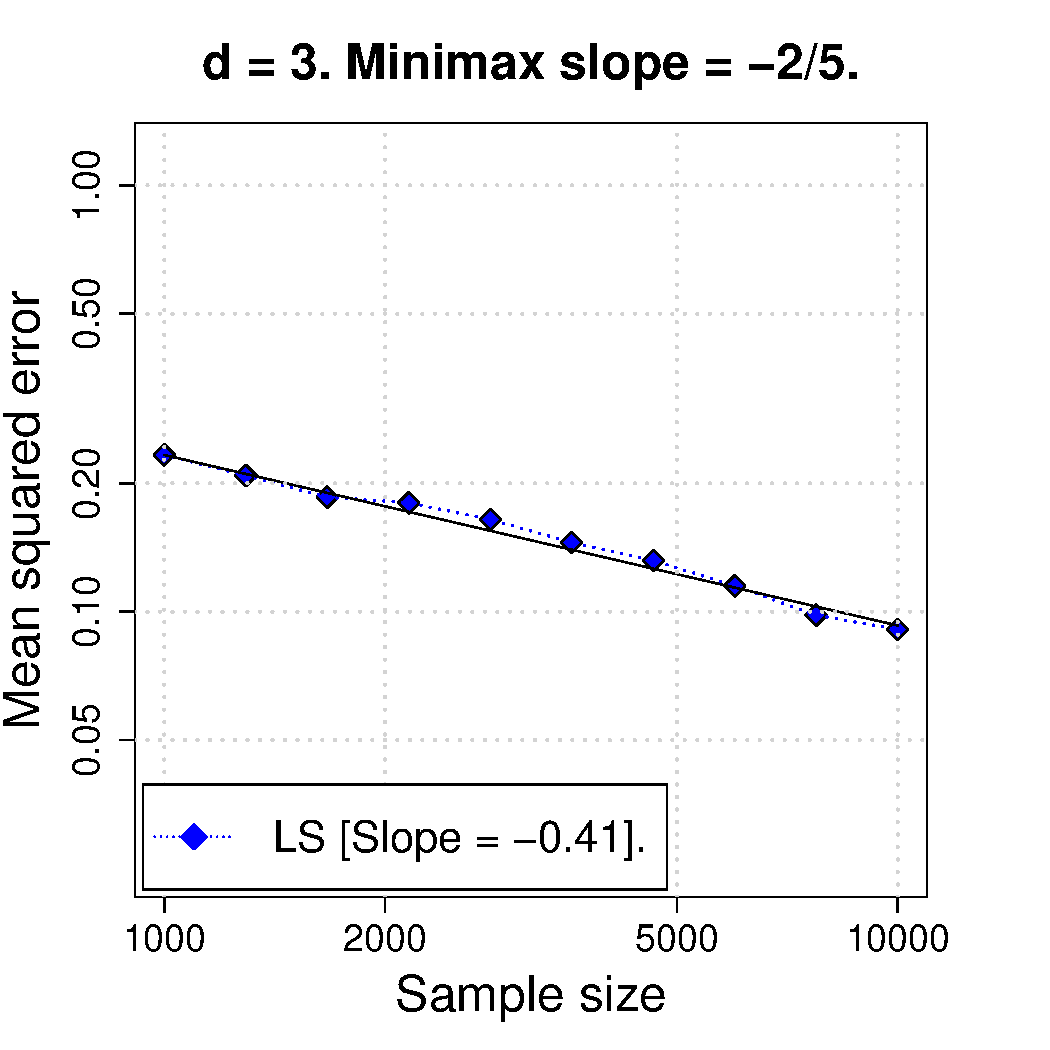
\includegraphics[width=.23\textwidth]{figures/cosine/mse_by_sample_size_3d.pdf}\\ 
	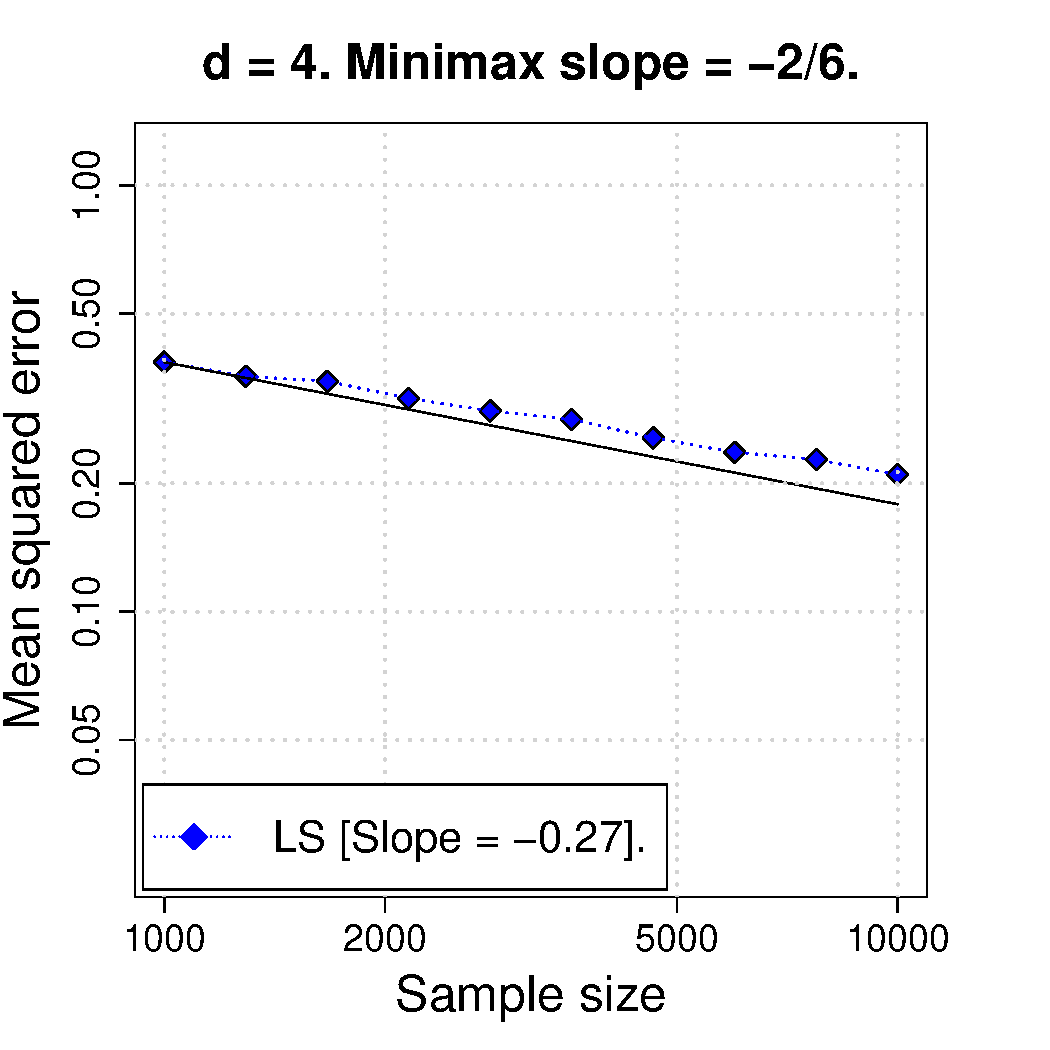
\includegraphics[width=.23\textwidth]{figures/cosine/mse_by_sample_size_4d.pdf}
	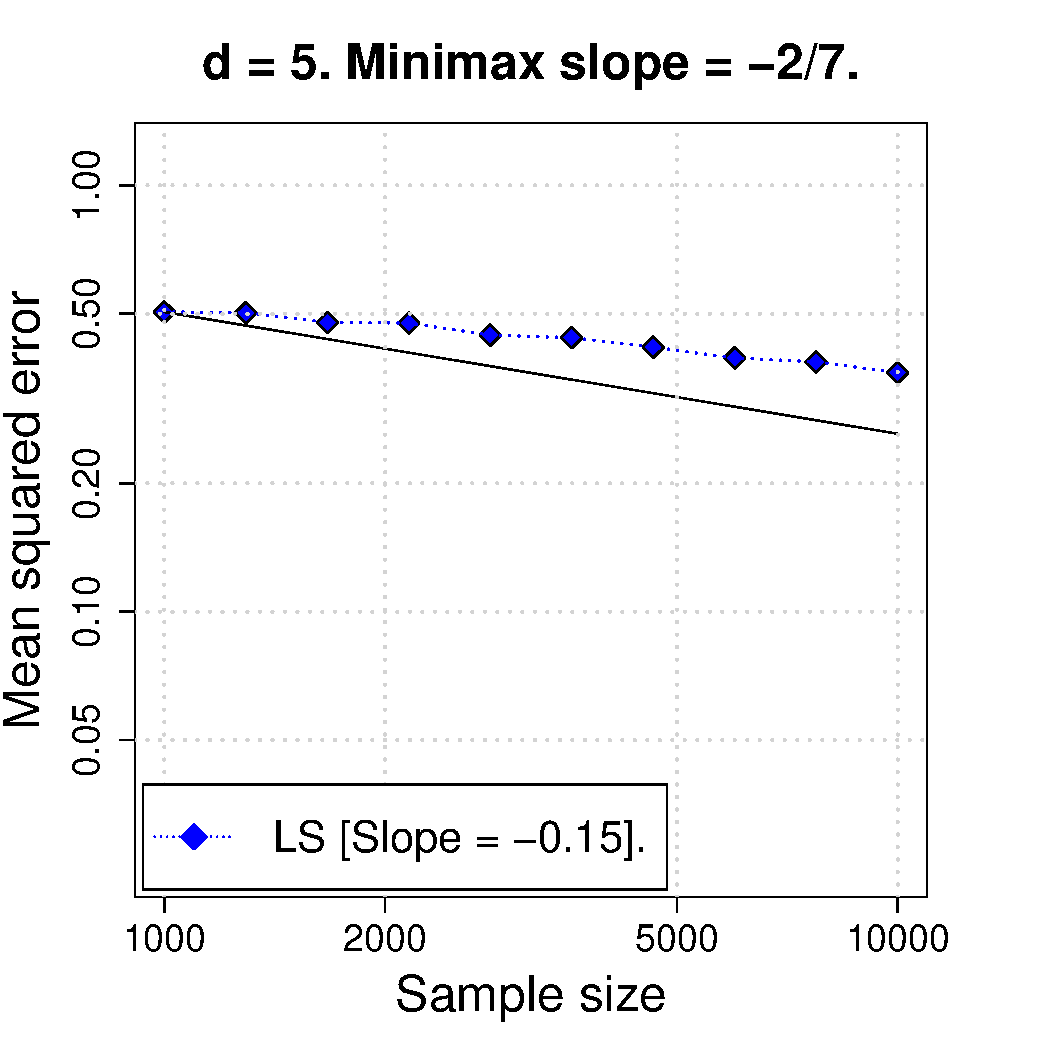
\includegraphics[width=.23\textwidth]{figures/cosine/mse_by_sample_size_5d.pdf}
	
	\caption{Mean squared error of Laplacian smoothing (\texttt{LS}) as a function of sample size $n$. Plots are on the log-log scale, MSE is averaged over 5 iterations, with Laplacian smoothing tuned for optimal MSE. The black line shows the minimax rate.}
	\label{fig:fig1}
\end{figure}

\paragraph{Testing error of Laplacian smoothing.}
Let us define a test using the statistic $\wh{T}$. For $b \geq 1$, set the threshold $\wh{t}_b$ as
\begin{equation*}
\wh{t}_{b} := \frac{1}{n}\sum_{k = 1}^{n} \frac{1}{\bigl(\rho \lambda_k + 1\bigr)^2} + \frac{2b}{n}\sqrt{\sum_{k = 1}^{n} \frac{1}{\bigl(\rho \lambda_k + 1\bigr)^4}},
\end{equation*}
where we recall $\lambda_k$ is the $k$th smallest eigenvalue of $\Lap_{n,r}$; the Laplacian smoothing test is simply $\wh{\varphi} := \1\bigl\{\wh{T} \leq \wh{t}_b\bigr\}$. (Clearly the test $\wh{\varphi}$ depends on $b$, but we suppress this notationally.) The number $b \geq 1$ is a tuning parameter selected by the user, with the choice made based on the tolerated level of Type I and Type II error. In fact, the threshold $\wh{t}_b$ is precisely the right choice to control the Type I error of $\wh{\varphi}$; as we show in our supplementary material,
\begin{equation}
\label{eqn:type_I_error}
\Ebb_0\bigl[\wh{\varphi}\bigr] \leq \frac{1}{b^2}.
\end{equation}
Theorem~\ref{thm:laplacian_smoothing_testing} establishes that this test also has small Type II error, uniformly over all $f_0$ separated from $0$ by at least the critical radius $\epsilon\bigl(H^1(\Xset,M)\bigr)$ given in~\eqref{eqn:sobolev_space_testing_critical_radius}. For this to hold, we will require a tight range of scalings for $r$.
\begin{enumerate}[label=(R\arabic*)]
	\setcounter{enumi}{1}
	\item 
	\label{asmp:ls_kernel_radius_testing}
	The neighborhood graph radius $r$ satisfies
	\begin{equation*}
	C_0\biggl(\frac{\log n}{n}\biggr)^{1/d} \leq r \leq M^{\frac{(d - 8)}{8 + 2d}}n^{\frac{d - 20}{32 + 8d}} \wedge c_0.
	\end{equation*}
\end{enumerate}
Note that when $d < 4$, if $M$ is not too large there always exists a choice of $r$ which satisfies~\ref{asmp:ls_kernel_radius_testing}.
\begin{theorem}
	\label{thm:laplacian_smoothing_testing}
	Let $f_0 \in H^1(\Xset,M)$ for $M \leq n^{(4 - d)/(4 + d)}$ and $d < 4$. Suppose that the neighborhood graph $G_{n,r}$ is computed with radius $r$ which satisfies~\ref{asmp:ls_kernel_radius_testing}, and the Laplacian smoothing test $\wh{\varphi}$ with $\rho = (nr^{d + 2})^{-1} n^{-4/(4 + d)} M^{-8/(4 + d)}$, and $b \geq 1$. For all $f_0$ such that
	\begin{equation}
	\label{eqn:laplacian_smoothing_testing}
	\bigl\|f_0\bigr\|_{\Leb^2(\Xset)}^2 \geq C b^2 M^{2d/(4 + d)} n^{-4/(4 + d)}
	\end{equation} 
	the Type II error is upper bounded:
	\begin{align*}
	& \Ebb_{f_0}\Bigl[1 - \wh{\varphi} \Bigr] \leq \\
	& C\biggl(\frac{1}{b}\Bigl[1 + n^{-d(4 + d)}M^{-2d/(4 + d)}\Bigr] + C_1n\exp\bigl(-c_1nr^d\bigr)\biggr).
	\end{align*}
\end{theorem}
A couple remarks:
\begin{itemize}
	\item As mentioned in Section~\ref{sec:problem_setup_and_background}, when $d \geq 4$ the Sobolev balls $H^1(\Xset,M)$ include quite irregular functions $f \not\in \Leb^4(\Xset)$. Proving tight lower bounds over such classes is non-trivial, and to the best of our knowledge such an analysis remains outstanding. On the other hand, if we explicitly assume that $f_0 \in \Leb^4(\Xset,M)$, then \cite{guerre02} show that the testing problem is characterized by the dimension-free lower bound $\epsilon^{2}(\Leb^4(\Xset,M)) \gtrsim n^{-1/2}$. Moreover, by training $\wh{f}$ to the interpolation limit, i.e. setting $\rho = 0$, the test $\wh{\varphi}$ achieves (up to constants) this lower bound. That is, for any $f_0 \in \Leb^4(\Xset,M)$ such that $\|f_0\|_{\Leb^2(\Xset)}^2 \geq C b^2n^{-1/2}$, we have both
	\begin{equation}
	\label{eqn:laplacian_smoothing_testing_low_smoothness}
	E_{f_0}\Bigl[1 - \wh{\varphi}\Bigr] \leq \frac{C(1 + M^4)}{b^2}
	\end{equation} 
	and $\Ebb_0[\wh{\varphi}] \leq 1/b^2$. These same results apply to $\wt{T}$, since when $d > 1$ the estimator $\wt{f}$ will interpolate the responses $Y_1,\ldots,Y_n$.
	\item To compute the data-dependent threshold $\wh{t}_b$, one must know each of the eigenvalues $\lambda_1,\ldots,\lambda_n$. Computing all $n$ of these eigenvalues is far more expensive---on the order of $n^3$ operations---than computing $\wh{T}$. That being said, in practice we would not recommend using $\wh{t}_b$ anyway, and would instead we make the standard recommendation to calibrate via a permutation test \citep{hoeffding1952}. 
\end{itemize}

\paragraph{Comparison with thin-plate splines.}
With some of our main results in hand, let us pause to offer some explanation of why Laplacian smoothing can be optimal in settings where thin-plate splines are not even consistent.  

First, we should make clear why this difference in performance is so surprising. As mentioned previously, the penalties in~\eqref{eqn:laplacian_smoothing} and~\eqref{eqn:thin_plate_spline} can be closely tied together: \cite{bousquet03} show that for any $f \in C^2(\Xset)$, 
\begin{equation}
\label{eqn:seminorm_consistency}
\begin{aligned}
\lim \frac{1}{n^2 r^{d + 2}} f^T \Lap_{n,r} f & = \int_{\Xset} f(x) \cdot \Delta_Pf(x) p(x) \,dx \\
& = \int_{\Xset} \|\nabla f(x)\|^2 p^2(x) \,dx
\end{aligned}
\end{equation}
in the above, the limit is as $n \to \infty$ and $r \to 0$, $\Delta_P$ is the (weighted) Laplace-Beltrami operator
\begin{equation*}
\Delta_Pf(x) := -\frac{1}{p} \dive\bigl(p^2\nabla f(x))
\end{equation*}
and the second equality follows from integration by parts.\footnote{Assuming $f$ satisfies Dirichlet boundary conditions.} To be clear, this argument does not formally imply that $\wh{f}$ and $\wt{f}$ are close---note that~\eqref{eqn:seminorm_consistency} holds for $f \in C^2(\Xset)$ whereas the domain of minimization in~\eqref{eqn:thin_plate_spline} is $H^1(\Xset)$---but it does seem to suggest that the two estimators should behave somewhat similarly. 

Of course, we know this is not the case: $\wh{f}$ and $\wt{f}$ look very different when $d > 1$. What is driving this difference? The key point is that the discretization imposed by the graph $G_{n,r}$---which seemed so problematic at first glance---turns out to be a blessing. The problem with~\eqref{eqn:thin_plate_spline} is that the function class $H^1(\Xset)$ is far too large when $d \geq 2$. This is meant in various related senses. From the Sobolev embedding theorem \cite{evans10}, we know that $H^1(\Xset)$ does not continuously embed into any H\"{o}lder space, and that $H^1(\Xset)$ is not an Reproducing Kernel Hilbert Space. More relevant to this context, by placing ``bump functions'' of arbitrarily small radius around each of the design points $X_1,\ldots,X_n$, one can interpolate the responses $Y_1,\ldots,Y_n$ in such a manner that forces the criterion in~\eqref{eqn:thin_plate_spline} to 0 \citep{green93}; the resulting estimator will clearly be inconsistent.

On the other hand~\eqref{eqn:laplacian_smoothing} is a finite dimensional (if growing linearly with $n$) problem---as a result $\wh{f}$ has far less capacity to overfit than does $\wt{f}$. Of course, discretization is not the only way to make the problem~\eqref{eqn:thin_plate_spline} more tractable: for instance, one could replace the penalty $\int_{\Xset} \|\nabla f(x)\|^2 \,dx$ by the stricter choice $\sup_{x \in \Xset} \|\nabla f(x)\|$,  or conduct the problem over some finite dimensional linear subspace of $H^1(\Xset)$ (i.e use a sieve). These solutions improve the statistical properties of $\wt{f}$ when $d > 1$ \citep{birge1993,birge1998,vandergeer2000}, but the first is computationally intractable, while the second requires the estimator to be specifically tailored to the domain $\Xset$, in stark contrast to $\wh{f}$.

\paragraph{Overview of analysis.}
The comparison with thin-plate splines highlights some surprising strengths of $\wh{f}$. Unfortunately, this comparison also precludes analyzing $\wh{f}$ by using~\eqref{eqn:seminorm_consistency} to establish a coupling between $\wh{f}$ and $\wt{f}$; we know this won't work, because we would like to prove tight error bounds on $\wh{f}$ in regimes where no such bounds exist for $\wt{f}$.

Instead we take a different approach, and directly analyze the error of $\wh{f}$ and $\wh{T}$ using a (conditional on $X_1,\ldots,X_n$) bias-variance decomposition. A standard calculation shows that
\begin{equation*}
\bigl\|\wh{f} - f_0\bigr\|_n^2 \leq \underbrace{\frac{2\rho}{n} \bigl(f_0^T \Lap_{n,r} f_0\bigr)}_{\textrm{bias}} + \underbrace{\frac{10}{n} \sum_{k = 1}^{n} \frac{1}{(\rho \lambda_k + 1)^2}}_{\textrm{variance}}
\end{equation*}
and likewise that $\wh{\varphi}$ has high power whenever
\begin{equation*}
\bigl\|f_0\bigr\|_n^2 \geq \underbrace{\frac{2\rho}{n} \bigl(f_0^T \Lap_{n,r} f_0\bigr)}_{\textrm{bias}} + \underbrace{\frac{4b}{n} \sqrt{\sum_{k = 1}^{n} \frac{1}{(\rho \lambda_k + 1)^4}}}_{\textrm{variance}}
\end{equation*}
Note that the bias and variance terms are each functionals of the random graph $G_{n,r}$, and so are themselves random. To upper bound them, we build on some recent works \citep{burago2014,trillos2019,calder2019} regarding the consistency of neighborhood graphs to establish the following two Lemmas. In the second of these Lemmas, we will assume
\begin{enumerate}[label=(R\arabic*)]
	\setcounter{enumi}{2}
	\item
	\label{asmp:radius1}
	The radius $r$ satisfies $C_0(\log n/n)^{1/d} \leq r \leq c_0$.
\end{enumerate}
and put $A_{n,r}(k) := \min\{nr^{d + 2}k^{2/d},nr^d\}$.

\begin{lemma}
	\label{lem:graph_sobolev_seminorm}
	For any $f \in H^1(\Xset)$, with probability at least $1 - \delta$, it holds that
	\begin{equation}
	\label{eqn:graph_sobolev_seminorm}
	f^T \Lap_{n,r} f \leq \frac{(1 + L_p)^2 \sigma_K}{\delta} n^2 r^{d + 2} |f|_{H^1(X)}^2.
	\end{equation}
\end{lemma}
\begin{lemma}
	\label{lem:neighborhood_eigenvalue}
	For any neighborhood graph radius $r$ which satisfies~\ref{asmp:radius1}, with probability at least $1 - C_1n\exp(-c_1nr^d)$ it holds that
	\begin{equation}
	\label{eqn:neighborhood_eigenvalue}
	c_2A_{n,r}(k) \leq \lambda_k \leq C_2A_{n,r}(k)~~\textrm{for all $2 \leq k \leq n$}
	\end{equation}
\end{lemma}

Lemma~\ref{lem:graph_sobolev_seminorm} gives a direct upper bound on the bias term. Lemma~\ref{lem:neighborhood_eigenvalue} results in a sufficient upper bound on the variance term whenever the neighborhood graph radius $r$ is \textit{sufficiently small}; precisely, when $r$ is upper bounded as in~\ref{asmp:ls_kernel_radius_estimation} (for estimation) or~\ref{asmp:ls_kernel_radius_testing} (for testing). The parameter $\rho$ is then tuned to minimize the sum of bias and variance, in the usual manner.

It is useful to give another perspective on our approach. When analyzing penalized least squares estimators such as $\wh{f}$ or $\wt{f}$ one typically assumes two properties: first, that the regression function $f_0$ lies in (or near) a ball in the normed space induced by the penalty, and second that this ball is reasonably small, e.g. as measured by metric entropy. In contrast, the Laplacian smoothing penalty induces a ball
\begin{equation*}
H^1(G_{n,r},M) := \{f: f^T \Lap_{n,r} f \leq M^2\}
\end{equation*}
that is data-dependent and random, and so we do not have access to either of the aforementioned properties \emph{a priori}; instead we must prove they hold with high probability. In this sense, our analysis is rather different than is typical in nonparametric regression.

\section{MANIFOLD ADAPTIVITY}
\label{sec:manifold_adaptivity}
The minimax rates $n^{-2/(2 + d)}$ (in estimation) and $n^{-4/(4 + d)}$ (in testing) suffer from the curse of dimensionality. However, in practice it is often reasonable to assume a \emph{manifold hypothesis}: roughly speaking, that the data $X_1,\ldots,X_n$ lie on a submanifold $\Xset$ of $\Rd$ that has intrinsic dimension $1 \leq m \leq d$. Under such an assumption, it is known \citep{bickel2007, ariascastro2018} that the optimal rates over $H^1(\Xset)$ now scale like $n^{-2/(2 + m)}$ (for estimation) and $n^{-4/(4 + m)}$ (for testing), which can be much smaller than the full-dimensional error rates when $m \ll d$. 

On the other hand, a theory has been developed~\citep{belkin03,belkin05,niyogi2013} establishing the the neighborhood graph $G_{n,r}$ can ``learn'' the manifold $\Xset$ in various senses, so long as $\Xset$ is locally linear. In this section, we contribute to this line of work by showing that under the manifold hypothesis, Laplacian smoothing achieves the sharper minimax rates over $H^1(\Xset)$.

\paragraph{Error rates with the manifold hypothesis.}
The conditions and results of this Section will be largely similar to the previous one, except with the ambient dimension $d$ replaced by the intrinsic dimension $m$. For the rest of this section we assume the following.
\begin{enumerate}[label=(P\arabic*)]
	\setcounter{enumi}{2}
	\item 
	\label{asmp:domain_manifold}
	The measure $P$ is supported on a compact, connected, smooth submanifold $\Xset$ of $\Reals^d$. The manifold $\Xset$ is of fixed dimension $1 \leq m \leq d$, is without boundary, and has positive reach \citep{federer1959}.
	\item 
	\label{asmp:density_manifold} $P$ has a density $p$ with respect to the volume form of $\Xset$ which is bounded away from $0$ and $\infty$,
	\begin{equation*}
	0 < p_{\min} \leq p(x) \leq p_{\max} < \infty
	\end{equation*}
	for all $x \in \Xset$. The density $p$ is Lipschitz with Lipschitz constant $L_p$.
\end{enumerate}
Under the assumptions~\ref{asmp:domain_manifold}, \ref{asmp:density_manifold} and~\ref{asmp:kernel}, and for a suitable range of $r$, the error bounds on the estimator $\wh{f}$ and test $\wh{\varphi}$ will depend on $m$ instead of $d$. 

\begin{enumerate}[label=(R\arabic*)]
	\setcounter{enumi}{3}
	\item 
	\label{asmp:ls_kernel_radius_estimation_manifold}
	The neighborhood graph radius $r$ satisfies
	\begin{equation*}
	C_3\biggl(\frac{\log n}{n}\biggr)^{1/m} \leq r \leq n^{\frac{-3}{(4 + 2m)}} M^{\frac{(m - 4)}{(4 + 2m)}} \wedge c_3.
	\end{equation*}
\end{enumerate}
\begin{theorem}
	\label{thm:laplacian_smoothing_estimation_manifold}
	Let $f_0 \in H^1(\Xset,M)$ with $m < 4$. Suppose that that the neighborhood graph $G_{n,r}$ is computed with a radius $r$ which satisfies~\ref{asmp:ls_kernel_radius_estimation_manifold},  and the Laplacian smoothing estimator $\wh{f}$ with $\rho = M^{-4/(2 + m)} (nr^{m + 2})^{-1} n^{-2/(2 + m)}$. With probability at least $1 - \delta -  C_4n\exp(-c_4nr^m) - \exp(-c M^{m/(2m + 4)} n^{m/(2+m)})$, it holds that
	\begin{equation*}
	\Bigl\|\wh{f} - f_0\Bigr\|_n^2 \leq \frac{C}{\delta} M^{2m/(2 + m)} n^{-2/(2 + m)}.
	\end{equation*}
\end{theorem}

We require the following range of $r$ for testing.
\begin{enumerate}[label=(R\arabic*)]
	\setcounter{enumi}{4}
	\item 
	\label{asmp:ls_kernel_radius_testing_manifold}
	The neighborhood graph radius $r$ satisfies
	\begin{equation*}
	C_3\biggl(\frac{\log n}{n}\biggr)^{1/m} \leq r \leq M^{\frac{(m - 8)}{8 + 2m}}n^{\frac{m - 20}{32 + 8m}} \wedge c_3.
	\end{equation*}
\end{enumerate}

\begin{theorem}
	\label{thm:laplacian_smoothing_testing_manifold}
	Let $f_0 \in H^1(\Xset,M)$ for $M \leq n^{(4 - m)/(4 + m)}$ and $m < 4$. Suppose that the neighborhood graph $G_{n,r}$ is computed with radius $r$ which satisfies~\ref{asmp:ls_kernel_radius_testing_manifold}, and the Laplacian smoothing test $\wh{\varphi}$ with $\rho = (nr^{m + 2})^{-1} n^{-4/(4 + m)} M^{-8/(4 + m)}$, and $b \geq 1$. If
	\begin{equation}
	\label{eqn:laplacian_smoothing_testing_manifold}
	\bigl\|f_0\bigr\|_{\Leb^2(\Xset)}^2 \geq C b^2 M^{2m/(4 + m)} n^{-4/(4 + m)},
	\end{equation} 
	the Type II error is upper bounded:
	\begin{align*}
	& \Ebb_{f_0}\Bigl[1 - \wh{\varphi} \Bigr] \leq \\
	& C\biggl(\frac{1}{b}\Bigl[1 + n^{-m(4 + m)}M^{-2m/(4 + m)}\Bigr] + C_4n\exp\bigl(-c_4nr^m\bigr)\biggr).
	\end{align*}
\end{theorem}
The proof of Theorems~\ref{thm:laplacian_smoothing_estimation_manifold} and~\ref{thm:laplacian_smoothing_testing_manifold} proceeds in a similar manner to that of Theorems~\ref{thm:laplacian_smoothing_estimation1} and~\ref{thm:laplacian_smoothing_testing}. The key difference is that in the manifold setting, the equations~\eqref{eqn:graph_sobolev_seminorm} and~\eqref{eqn:neighborhood_eigenvalue} that we use to upper bound bias and variance will hold with $d$ replaced by $m$.

We emphasize that very little about $\Xset$ need be known for Theorems~\ref{thm:laplacian_smoothing_estimation_manifold} and~\ref{thm:laplacian_smoothing_testing_manifold} to hold. Indeed, all that is needed is the intrinsic dimension $m$--- in order to properly tune $r$ and $\rho$--- and otherwise $\wh{f}$ and $\wh{\varphi}$ are computed without regard to $\Xset$. In contrast, the penalty in~\eqref{eqn:thin_plate_spline} would have to be specially tailored to work in this setting, revealing another advantage of Laplacian smoothing compared to thin-plate splines.

\section{DISCUSSION}
\label{sec:discussion}
In this work, we have shown that Laplacian smoothing over a neighborhood graph is optimal for both estimation and goodness-of-fit testing problems.

There are still several extensions we feel are worth pursuing. In practice, it is more common to use $k$NN graphs than neighborhood graphs, due to the guaranteed connectivity and sparsity of the former; we suspect that by building on the work of~\cite{calder2019}, one can show that our main results all hold when the $k$NN graph is used. In another direction, one can also generalize Laplacian smoothing by replacing the penalty $f^T \Lap_{n,r} f$ with $f^T \Lap_{n,r}^k f$ for some $k > 1$. The hope is that this adapted procedure would be minimax optimal over the previously mentioned higher-order Sobolev classes $H^k(\Xset)$. In the very special case of $k = 2$ and $d \leq 2$, we can show that this is indeed the case, but the general story--for all combinations of $k$ and $d$---remains beyond our reach. 

\bibliographystyle{plainnat}
\bibliography{../../../graph_testing_bibliography} 

\end{document}